\begin{figure*}[!t]
\centering
\begin{tabular}{cccc}
\subfloat[1 worker by processing stage]{
  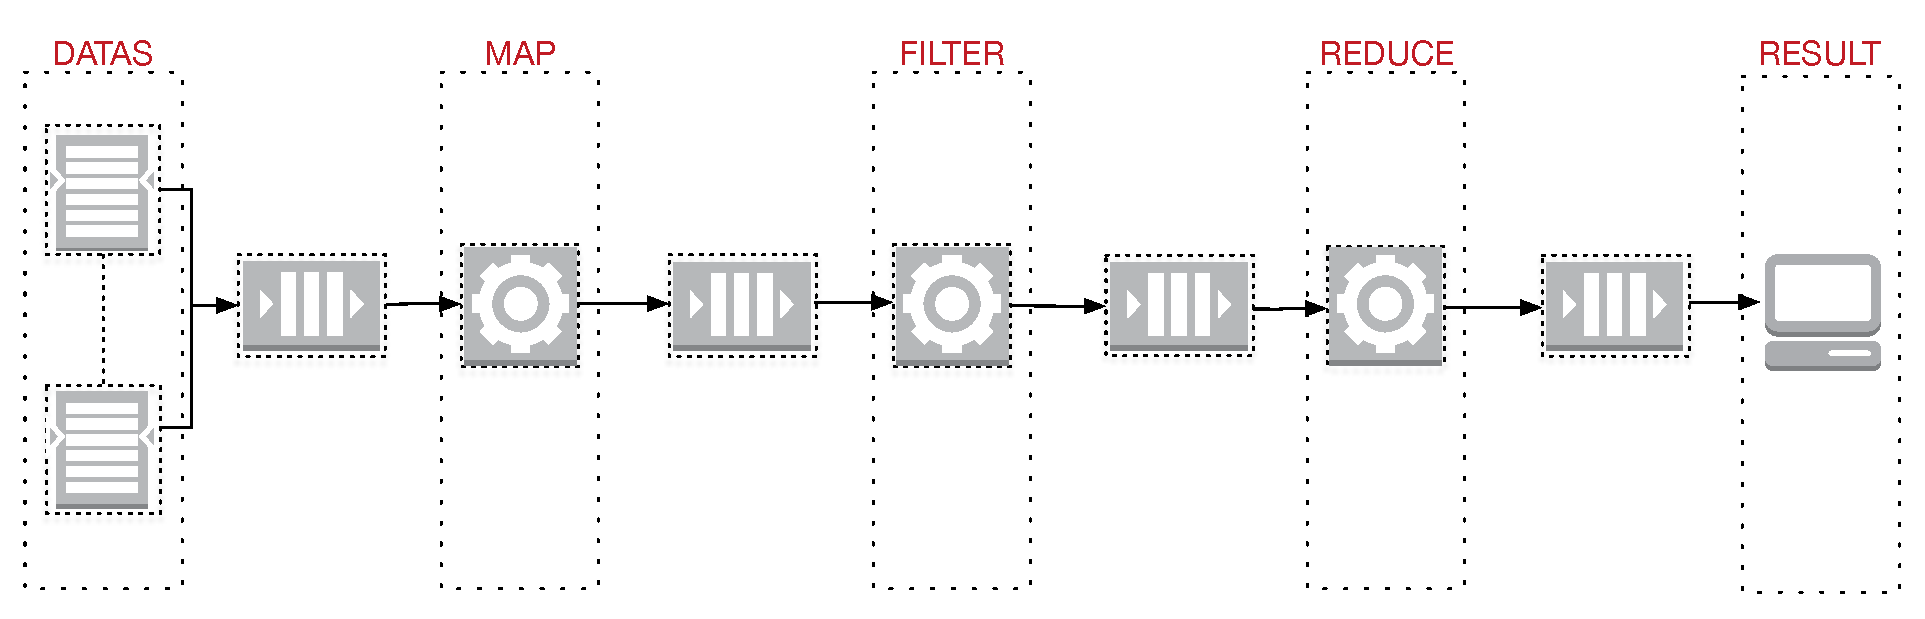
\includegraphics[width=0.3\textwidth]{images/pipeline-1worker.pdf}
} &
\subfloat[Throughput without SGX]{
  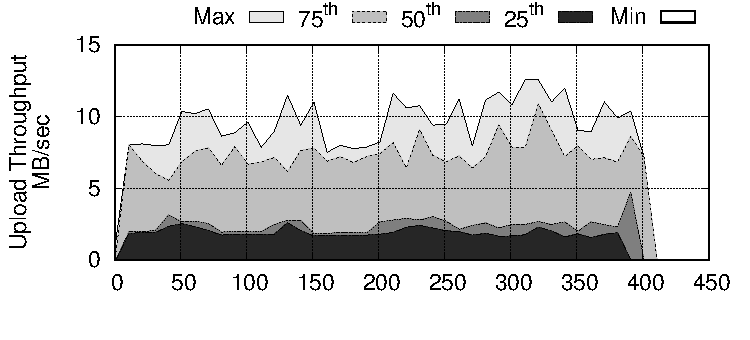
\includegraphics[width=0.3\textwidth]{plots/secure_streams/throughput/tput_tx_percentiles_1-workers.pdf}
} &
\subfloat[Throughput with SGX]{
  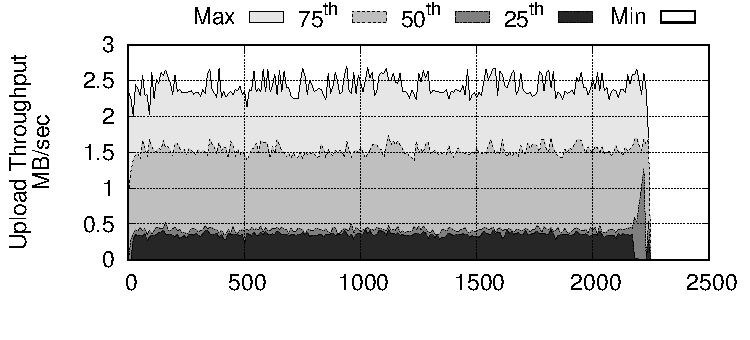
\includegraphics[width=0.3\textwidth]{plots/secure_streams/throughput/tput_tx_percentiles_1-workers-fullsgx.pdf}
}\cr
\subfloat[2 workers by processing stage]{
  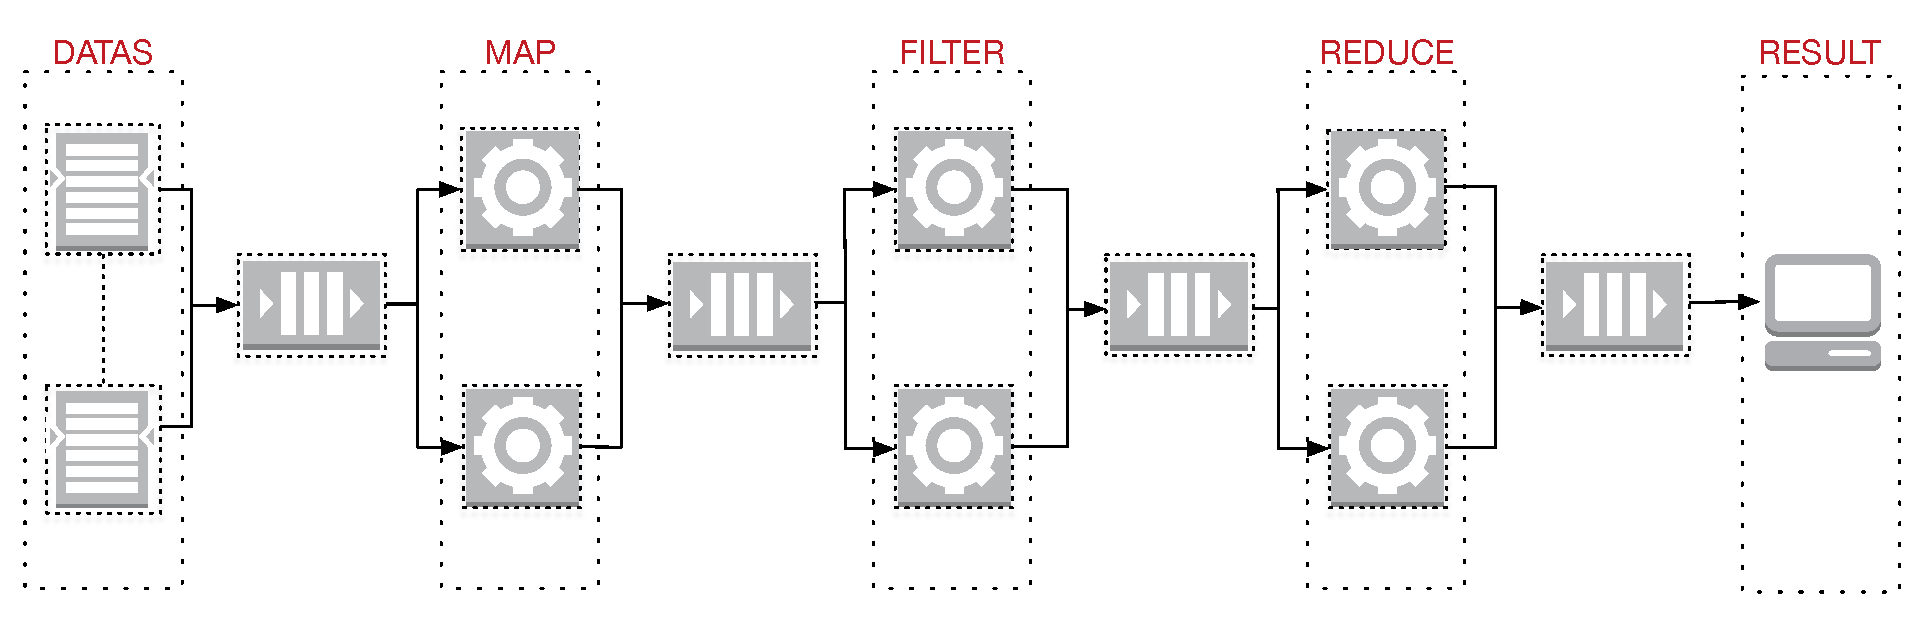
\includegraphics[width=0.3\textwidth]{images/pipeline-2workers.pdf}
} &
\subfloat[Throughput without SGX]{
  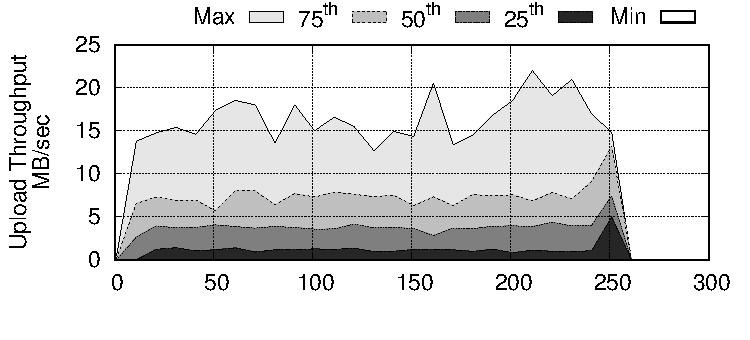
\includegraphics[width=0.3\textwidth]{plots/secure_streams/throughput/tput_tx_percentiles_2-workers.pdf}
} &
\subfloat[Throughput with SGX]{
  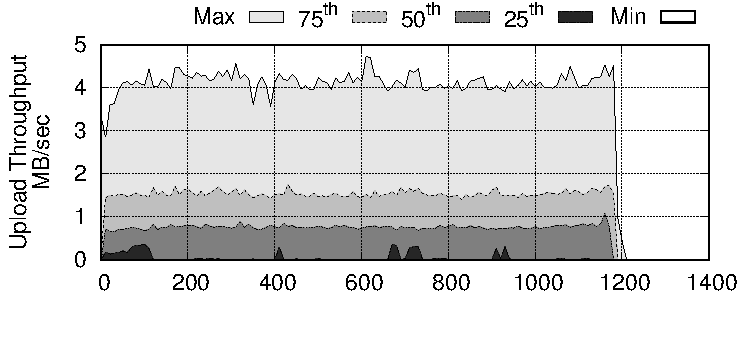
\includegraphics[width=0.3\textwidth]{plots/secure_streams/throughput/tput_tx_percentiles_2-workers-fullsgx.pdf}
}\cr
\subfloat[4 workers by processing stage]{
  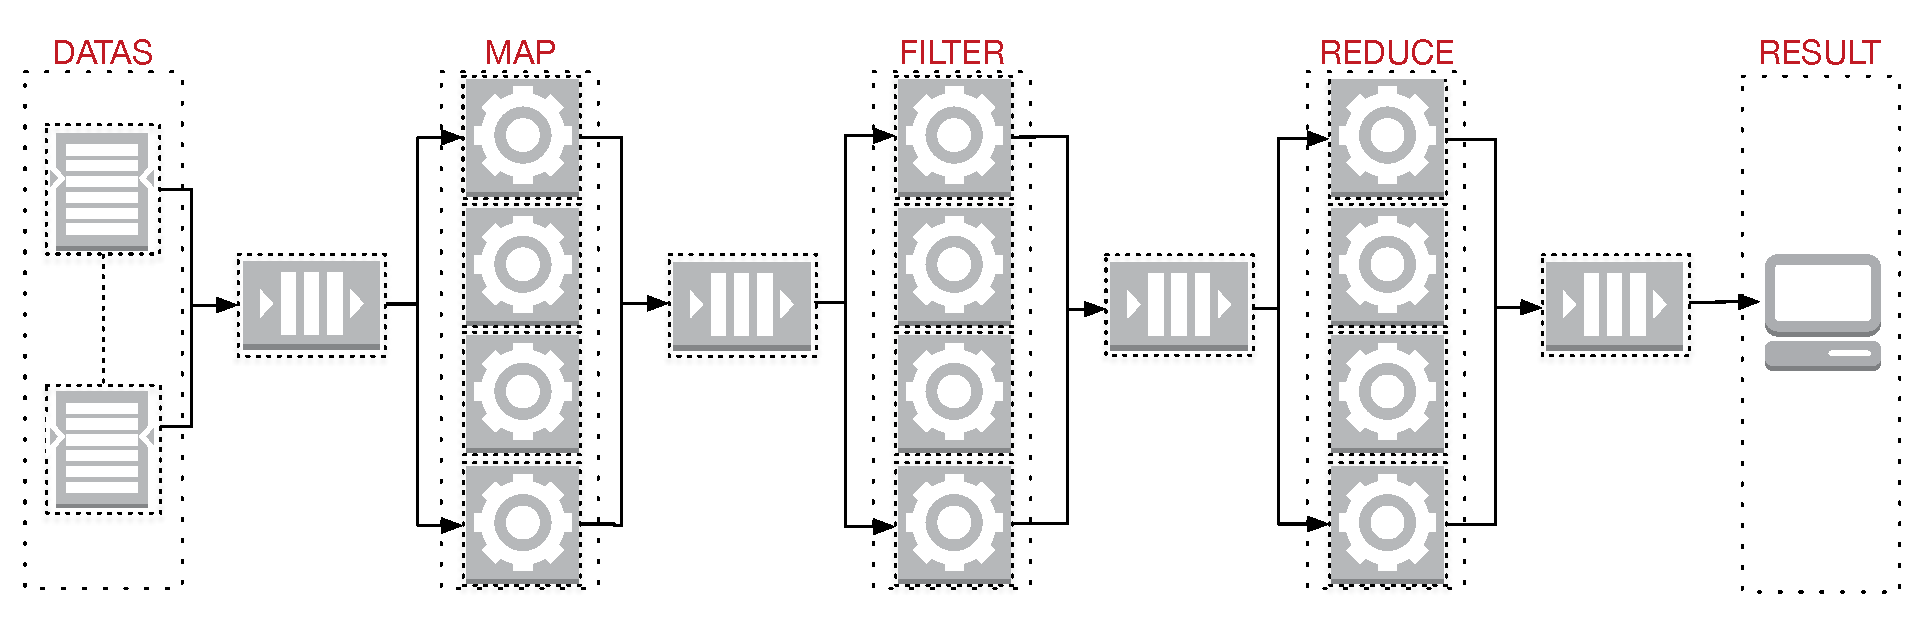
\includegraphics[width=0.3\textwidth]{images/pipeline-4workers.pdf}
} &
\subfloat[Throughput without SGX]{
  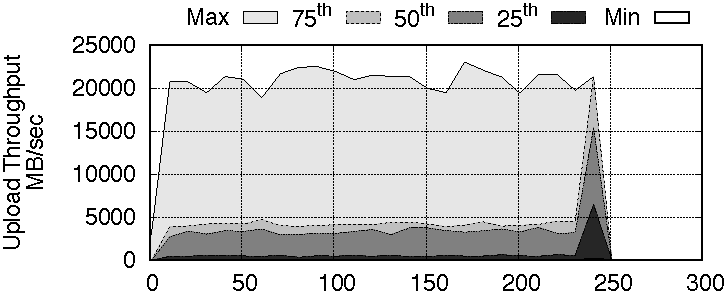
\includegraphics[width=0.3\textwidth]{plots/secure_streams/throughput/tput_tx_percentiles_4-workers.pdf}
} &
\subfloat[Throughput with SGX]{
  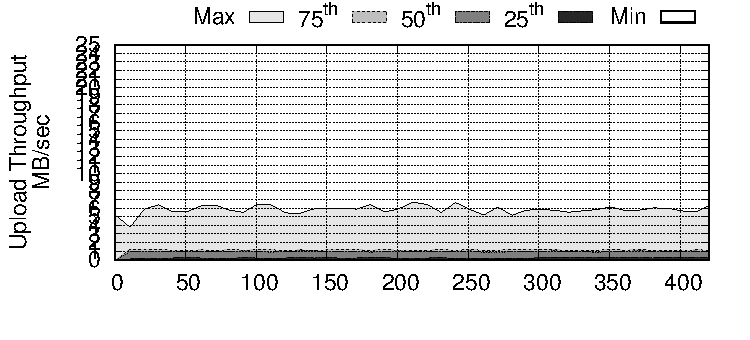
\includegraphics[width=0.3\textwidth]{plots/secure_streams/throughput/tput_tx_percentiles_4-workers-fullsgx.pdf}
}
\end{tabular}
\caption{Throughput camparison between normal processing and SGX processing}
\end{figure*}
